\subsection{Glyphs: \glyph{Subunits}}
\label{sec:subunit}

A complex is formed by the non-covalent binding of two or more entities, that become the subunits of the complex.
In \PD, the composition of a complex may be described using \glyph{subunit} glyphs, that are auxiliary units decorating \glyph{complexes}.
\glyph{Subunits} do not represent or mimic entity pools~(\sect{EPNs}) and may only be used to represent the subunits included in a complex.
The example in \fig{complexSubunits} illustrates the use of \glyph{subunits} to describe the composition of a complex.
It also shows how the same complex can be represented without decorating \glyph{subunits}.

The SBGN \PD defines nine different \glyph{subunit} glyphs, each representing a different type of bio-molecular (sub)-entity.
The five main \glyph{subunits} are the \glyph{unspecified entity subunit}, \glyph{macromolecule subunit}, \glyph{simple chemical subunit}, \glyph{nucleic acid feature subunit}, and \glyph{complex subunit}.
This latter \glyph{subunit} allows representing complexes formed of other complexes.
The remaining four \glyph{subunits} are multimeric: \glyph{multimer of macromolecules subunit}, \glyph{multimer of simple chemicals subunit}, \glyph{multimer of nucleic acid feature subunit}, and \glyph{multimer of complexes subunit}.

\begin{glyphDescription}

\glyphSboTerm
Not applicable.

\glyphIncoming
None.

\glyphOutgoing
None.

\glyphContainer
Each \glyph{subunit} is represented by its own shape depending on its bio-molecular nature, as shown in \tab{subunit_containers}.
Those shapes are the same as those used to represent entity pools~(\sect{EPNs}).

\glyphLabel
A \glyph{subunit} is identified by a label that is a string of characters that can be distributed on several lines to improve readability.
The centre of the label must be placed on the centre of the container.
The label may extend outside of the container.

\glyphAux A \glyph{subunit} may carry auxiliary units, depending on its type.

A \glyph{macromolecule}, \glyph{nucleic acid feature}, or \glyph{complex subunit} can carry one or more \glyph{state variables} that add information about its state (\sect{stateVariable}).
The state of such a \glyph{subunit} is defined as the list of all its \glyph{state variables}.

A \glyph{macromolecule}, \glyph{simple chemical}, \glyph{nucleic acid feature}, or \glyph{complex subunit} can carry one or more \glyph{units of information} (\sect{unitInfo}).
These can characterize a domain, such as a binding site.
Particular \glyph{units of information} are available for describing the material type (\sect{material-types-cv}) and conceptual type (\sect{conceptual-types-cv}) of such a \glyph{subunit}.

\end{glyphDescription}

\begin{table}[h]
\begin{tabu}{X[c,m]X[c,m]X[c,m]X[c,m]}
    \toprule
    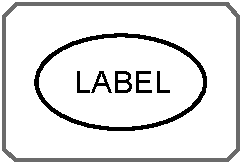
\includegraphics[scale=0.8, valign=m]{images/build/unspecified_subunit.pdf} & 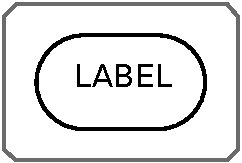
\includegraphics[scale=0.8, valign=m]{images/build/simple_chemical_subunit.pdf} & 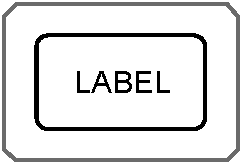
\includegraphics[scale=0.8, valign=m]{images/build/macromolecule_subunit.pdf} & 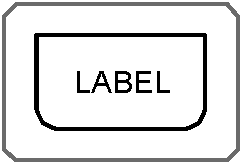
\includegraphics[scale=0.8, valign=m]{images/build/genetic_subunit.pdf}\\[0.2cm]
    \glyph{unspecified entity subunit} & \glyph{simple chemical subunit} & \glyph{macromolecule subunit} & \glyph{nucleic acid feature subunit}\\[0.5cm]
    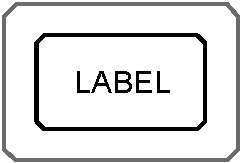
\includegraphics[scale=0.8, valign=m]{images/build/complex_subunit.pdf} & 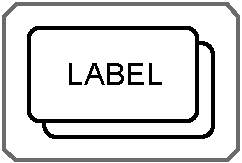
\includegraphics[scale=0.8, valign=m]{images/build/macromolecule_multimer_subunit.pdf} & 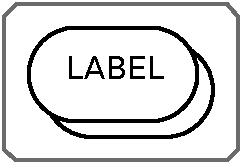
\includegraphics[scale=0.8, valign=m]{images/build/simple_chemical_multimer_subunit.pdf} & 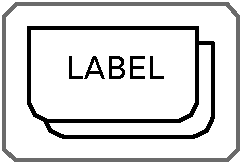
\includegraphics[scale=0.8, valign=m]{images/build/genetic_multimer_subunit.pdf}\\[0.2cm]
    \glyph{complex subunit} & \glyph{multimer of macromolecules subunit} & \glyph{multimer of simple chemicals subunit} & \glyph{multimer of nucleic acid feature subunit}\\[0.5cm]
    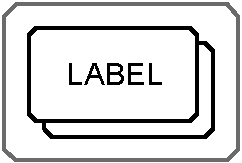
\includegraphics[scale=0.8, valign=m]{images/build/complex_multimer_subunit.pdf} &  &  & \\[0.2cm]
    \glyph{multimer of complexes subunit} & & & \\
    \bottomrule
\end{tabu}
\caption{The \PD glyphs for the different types of \glyph{subunits}.
Each \glyph{subunit} decorates a \glyph{complex}.}
\label{tab:subunit_containers}
\end{table}

\begin{figure}[htb]
  \centering
  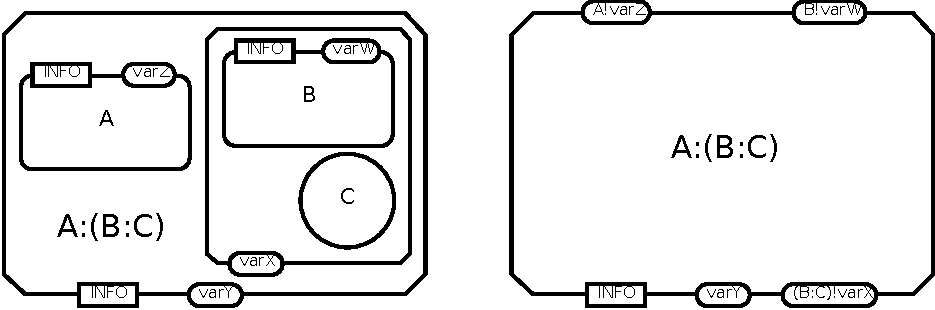
\includegraphics[scale=0.8]{images/build/complex.pdf}
  \caption{Both these complex glyphs are equivalent.
      The complex on the left is described using \glyph{subunit} decorators.
      The complex on the right depicts the same information, without explicitly representing those subunits, that are only suggested by the label of the \glyph{complex}.
      However, their states are represented using \glyph{state variables} decorating the \glyph{complex}.}
  \label{fig:complexSubunits}
\end{figure} 
